%==============================================================================
%  Verification-First Generation of First Examination Report Responses
%  IEEE conference format (IEEEtran, two-column)
%
%  Build:  pdflatex paper-fer-response
%          pdflatex paper-fer-response      % twice, for cross-references
%
%  Requires: IEEEtran.cls (standard in TeX Live / MiKTeX)
%            figures/fig1-pipeline.png  (regenerate: node scripts/paper-figure.js)
%==============================================================================
\documentclass[conference]{IEEEtran}
\IEEEoverridecommandlockouts

\usepackage{cite}
\usepackage{amsmath,amssymb}
\usepackage{graphicx}
\usepackage{textcomp}
\usepackage{booktabs}
\usepackage{array}
\usepackage{url}
\usepackage[T1]{fontenc}
\usepackage[utf8]{inputenc}

\newcommand{\code}[1]{\texttt{\small #1}}

\begin{document}

\title{Verification-First Generation of First Examination\\Report Responses: An LLM Architecture for\\Indian Patent Prosecution}

\author{
\IEEEauthorblockN{[Author 1]}
\IEEEauthorblockA{\textit{[Department]}\\
\textit{[Institution]}\\
[City, Country]\\
[email]}
\and
\IEEEauthorblockN{[Author 2]}
\IEEEauthorblockA{\textit{[Department]}\\
\textit{[Institution]}\\
[City, Country]\\
[email]}
\and
\IEEEauthorblockN{[Author 3]}
\IEEEauthorblockA{\textit{[Department]}\\
\textit{[Institution]}\\
[City, Country]\\
[email]}
}

\maketitle

\begin{abstract}
Every patent application in India receives a First Examination Report (FER), a statutory letter in which the Controller raises objections on novelty, inventive step, patentable subject matter, sufficiency, clarity and procedural compliance. The applicant must answer every objection within six months, and a single unanswered objection can cost the application. Drafting that reply is slow, repetitive and highly consequential, which makes it an attractive target for large language models (LLMs). It is also a setting in which the standard failure mode of LLMs---fluent, confident, unsupported assertion---is not a nuisance but a professional misrepresentation to a public authority. We present a deployed system that generates filing-ready FER replies while structurally preventing that failure. Its central principle is that \emph{a prompt instruction is a request, whereas a post-hoc check in code is a guarantee}, and that only the second may be trusted. The system runs a seven-stage pipeline in which every generative stage is immediately followed by a deterministic verifier: examiner quotations must substring-match the report; claim-chart passages must substring-match the cited document; every word inserted by an amendment must be traceable to the specification as filed; case law is restricted to a per-objection whitelist; and formal objections never reach a model at all. Jurisdiction-specific law is held entirely in a validated JSON profile, so no source file branches on a country code. A retrieve-per-need context strategy reads the full specification exactly once, which reduces the estimated per-case input budget by roughly an order of magnitude relative to a naive prompt-stuffing design. Nothing is filed automatically: a blocking compliance lint of twenty deterministic checks stands between the draft and the exported document. We describe the architecture, the verification layer in detail, the cost model, and the regression suite that protects the invariants, and we discuss what such a system can and cannot responsibly claim.
\end{abstract}

\begin{IEEEkeywords}
patent prosecution, office action response, large language models, retrieval-augmented generation, hallucination mitigation, evidence grounding, legal informatics, intellectual property law, human-in-the-loop systems, Indian Patents Act
\end{IEEEkeywords}

%==============================================================================
\section{Introduction}

\subsection{The First Examination Report}

Indian patent prosecution is organised around a single document. After a request for examination, the Controller issues a \textbf{First Examination Report} under Sections 12 and 13 of the Patents Act, 1970 \cite{act1970}. The FER is a structured letter. Part~I records administrative findings; Part~II carries the detailed substantive observations---objections on novelty (Section 2(1)(j)), inventive step (Section 2(1)(ja)), non-patentable subject matter (Section 3, most often 3(d) and 3(k)), sufficiency and clarity (Section 10), and unity (Section 10(5)); Part~III lists formal requirements such as an updated Form~3 statement under Section 8, biological-source declarations, and National Biodiversity Authority approvals.

The reply is governed by a hard clock. Under Rule 24B(5) of the Patents Rules, 2003, the application must be put in order for grant within \textbf{six months of the FER date}, extendable by three months on a Form~4 request that, following the Patents (Amendment) Rules, 2024, may be filed at any time within nine months of that date \cite{rules2003}. Failure is not recoverable in the ordinary course: the application is deemed abandoned under Section 21(1), and no statutory revival exists.

Two properties of this task make it unusually demanding. First, \textbf{completeness is mandatory}. The reply must answer every objection under the Controller's own numbering; an objection that is silently dropped is the single worst defect a reply can carry. Second, \textbf{amendments are tightly constrained}. Section 59(1) permits amendment only by way of disclaimer, correction or explanation, forbids new matter, and requires that amended claims fall wholly within the scope of the claims before amendment. In practice the Controller expects each amendment to be supported by an identified location in the specification as filed. The functional equivalent in Europe is Article 123(2) EPC \cite{epc}, and the same logic drives the United States prohibition on new matter under 35 U.S.C. \S132(a) \cite{usc132}.

\subsection{Why LLMs, and Why Not LLMs Alone}

An FER reply is largely a document-grounded writing task: read the objection, read the cited prior art, compare it with the claims, decide whether to argue or amend, and write formal correspondence in a fixed house style. LLMs are genuinely good at each of those sub-tasks in isolation, and the volume of routine prosecution work in India---where a large share of filings are handled by small firms under fee pressure---makes automation economically attractive.

The difficulty is that the same properties that make an LLM useful here make it dangerous here. Three failure modes are decisive.

\begin{enumerate}
\item \textbf{Fabricated evidence.} A model asked to quote the examiner, or to quote a cited patent, will often produce a plausible sentence that appears nowhere in either document. Legal hallucination is not a marginal phenomenon; controlled studies of general-purpose models on legal queries report hallucination rates between 58\,\% and 88\,\% depending on task and jurisdiction \cite{dahl2024}, and even purpose-built commercial legal research tools have been shown to produce unsupported outputs at material rates \cite{magesh2025}.
\item \textbf{Unsupported amendment basis.} A model can assert that an inserted limitation is supported at paragraph [0038] with complete confidence and no relationship to the actual text. Under Section 59 this is not a stylistic defect; it is an added-matter objection waiting to happen, and in the worst case a ground of revocation under Section 64(1)(o).
\item \textbf{Asserted compliance.} A model answering a Section 8 objection will readily write ``the updated Form~3 has been filed herewith.'' If it has not been filed, the attorney has just made a false statement to the Controller under their own signature.
\end{enumerate}

These are not problems that better prompting solves. They are problems of \textbf{verification}, and verification of a generated assertion against a source document is a task that ordinary deterministic code performs far more reliably than any model.

\subsection{Contributions}

This paper describes an \emph{Office Action Studio} module deployed inside a commercial patent-workflow platform, focusing on its Indian FER configuration. Our contributions are:

\begin{enumerate}
\item \textbf{A verification-first pipeline architecture} (Section~\ref{sec:verification}) in which each of seven processing stages is a pair---one generative call followed by one deterministic guard---and in which no generated assertion reaches the filed document without an anchor that code has checked.
\item \textbf{A grounding primitive} (\code{verifyQuote}) tuned for real PDF-extracted text: strict exact matching for short spans, and consecutive word-bigram coverage above a $0.85$ threshold for long ones, which absorbs optical-character-recognition noise while still rejecting invented sentences.
\item \textbf{A Section 59 added-matter guard implemented as a database query filter} rather than a prompt instruction, so that post-filing material is structurally incapable of becoming amendment basis, combined with a word-coverage test on every inserted span.
\item \textbf{Two complementary consistency checks}---a full-document absence scan that corrects claim-chart verdicts formed on truncated evidence, and a contradiction lint that catches drafted prose asserting the opposite of its own chart.
\item \textbf{A jurisdiction-as-data design} in which all local law lives in a schema-validated JSON profile, so that supporting a new patent office is an authoring task rather than an engineering task.
\item \textbf{A retrieve-per-need context strategy} that reads the full specification exactly once and thereafter serves stages from a cached digest plus top-$K$ vector retrieval, giving an estimated order-of-magnitude reduction in per-case input tokens.
\item \textbf{A blocking compliance gate} of twenty deterministic checks that a draft must pass before any document can be exported.
\end{enumerate}

%==============================================================================
\section{Related Work}

\textbf{Patent-domain natural language processing.} Automated patent analysis has a long history, surveyed comprehensively by Krestel \emph{et al.} \cite{krestel2021}. Generative work has concentrated on drafting rather than prosecution: Lee and Hsiang demonstrated claim generation by fine-tuning a general language model \cite{lee2020}, and Casola and Lavelli examined summarisation and simplification of patent text \cite{casola2022}. Prior-art retrieval has attracted the most sustained attention, including open efforts that frame novelty search as semantic retrieval. Office-action response generation is comparatively unexplored in the literature, and the Indian FER---with its distinctive Section 3 subject-matter grounds and its Section 59 amendment discipline---has received almost no published treatment.

\textbf{Retrieval-augmented generation.} Grounding generation in retrieved documents is the standard mitigation for hallucination \cite{lewis2020}, and retrieval has been shown to reduce unsupported assertions substantially in dialogue settings \cite{shuster2021}. Our design uses retrieval but does not rely on it as the safety mechanism. In conventional RAG, retrieved text is \emph{context} and the model is trusted to use it faithfully. Here, retrieved text is the \emph{only admissible substrate}, and---more importantly---the model's use of it is re-checked afterwards by code that does not consult the model. This distinction matters: RAG reduces the probability that a model fabricates, whereas a post-hoc substring check reduces the probability that a fabrication survives to the filed document.

\textbf{Hallucination in legal applications.} Dahl \emph{et al.} profile legal hallucination systematically and observe that models are most confident precisely where they are least reliable, particularly on lower-court and jurisdiction-specific material \cite{dahl2024}. Magesh \emph{et al.} extend this to retrieval-augmented commercial legal tools and find that grounding alone does not eliminate the problem \cite{magesh2025}. Both results argue directly for our position: the mitigation must be an artifact-level check, not an author-level instruction \cite{ji2023}.

\textbf{Verification of generated output.} Our guards belong to the same family as self-consistency and post-hoc verification techniques, but differ in a way we consider essential. Verification here is performed by string algorithms and database predicates rather than by a second model call. A verifier that is itself a language model shares the failure distribution of the generator; a substring test does not.

%==============================================================================
\section{Design Principles}

Three principles govern the module. They are stated here because every subsequent design decision follows from them.

\subsection{Jurisdiction Logic Is Data, Never Code}

No file in the module may branch on a country code. All local law---the instruments an office issues, its deadline rules, its objection vocabulary and statutory bases, its doctrinal reasoning steps, its amendment scope rule, its permitted authorities and its reply layout---lives in an \code{officeActionProfile} block inside a per-country JSON file, validated by a schema. Adding a jurisdiction is therefore an authoring exercise: write the profile, pass structural and semantic validation, pass a readiness check, synchronise it to the database, and activate it. This keeps the engine small and auditable, and it prevents the slow accretion of jurisdiction-specific conditionals that typically makes legal software unmaintainable.

\subsection{Every Assertion Is Anchored, and the Anchor Is Checked in Code}

The module states this as a rule about trust: \emph{a prompt instruction is a request; a post-hoc string check is a guarantee.} Both are used, but only the second is relied upon. Consequently, prompts do carry anti-fabrication instructions---copy verbatim, mark a feature as \code{NOT\_DISCLOSED} rather than inventing disclosure, cite specification basis or state plainly that none exists, never claim a form has been filed---and those instructions are treated as belt rather than braces. The guards described in Section~\ref{sec:verification} are what actually holds.

\subsection{Read the Invention Once}

The full specification is sent to a model exactly once per case, during a digest pass. Every subsequent stage operates on that cached digest plus a small set of vector-retrieved paragraphs. This is presented in Section~\ref{sec:cost} as a cost measure, but it is equally a quality measure: a stage that receives four thousand tokens of targeted context reasons better than one that receives fifty thousand tokens of everything.

%==============================================================================
\section{System Architecture}

\subsection{Layered Structure}

The module is organised into five layers, summarised in Table~\ref{tab:layers}. Supporting infrastructure includes a single LLM entry point, a context-budget and retrieval service, a pure document-normalisation library, a calendar engine, a doctrine renderer and the profile schema.

\begin{table*}[t]
\caption{Layered structure of the FER response module}
\label{tab:layers}
\centering
\renewcommand{\arraystretch}{1.25}
\begin{tabular}{@{}>{\raggedright\arraybackslash}p{0.16\textwidth}>{\raggedright\arraybackslash}p{0.78\textwidth}@{}}
\toprule
\textbf{Layer} & \textbf{Responsibility} \\
\midrule
Interface & Case list and a workspace comprising a deadline strip, an objection rail, a four-tab workbench (Objection / Evidence / Strategy / Draft), and a docked source viewer \\
HTTP & Nine endpoints covering case creation, document ingestion, citation management, objection triage, run control, draft editing and export \\
Orchestration & Intake orchestration, the reply-preparation pipeline, and a database-lease job worker \\
Stages & Eight stage modules, each structured as \emph{generative call $\rightarrow$ deterministic guard $\rightarrow$ typed result} \\
Output & Deterministic reply assembly, a blocking compliance lint, a filing-grade DOCX renderer, an HTML preview sharing the same block model, and outcome notification \\
\bottomrule
\end{tabular}
\end{table*}

\subsection{The Jurisdiction Profile}

The profile is the module's configuration surface and its legal specification. Its principal keys are:

\begin{itemize}
\item \code{instruments[]}---the document types the office issues, each with detection hints that drive \emph{deterministic} instrument recognition, and the metadata fields the parser should extract. The Indian profile declares three: FER, Subsequent Examination Report, and Hearing Notice.
\item \code{timeline.deadlines[]}---rules of the form \{trigger, period, extension, consequence\} expressed in ISO-8601 durations. The Indian profile encodes the Rule 24B(5) six-month reply period with its Form~4 extension and nine-month request window, the three-month updated Form~3 obligation under Rule 12(3) as amended in 2024, and the fifteen-day post-hearing written-submissions window under Rule 28(7).
\item \code{objections[]}---a mapping from a canonical code to the local statute, detection hints, response type, sub-types, doctrine key, action checklist, standard reply sentence, and a \textbf{case-law whitelist}. The Indian profile declares eight objection families and expands eligibility into seven Section 3 sub-clauses (3(k), 3(d), 3(e), 3(c), 3(f), 3(i), 3(m)).
\item \code{doctrines\{\}}---ordered reasoning steps a drafter must follow, with leading authorities \cite{novartis,ferid,cri2017}.
\item \code{amendments}---the scope rule quoted verbatim from Section 59(1), the basis requirement, and the marked/clean copy convention.
\item \code{response.skeleton[]}---the ordered section identifiers, which are literally the switch in the assembly function. The Indian skeleton runs: address block, subject line, preliminary submissions, objection-wise reply, marked amended claims, clean amended claims, conclusion and prayer, signature block.
\item \code{prompts\{\}}---per-stage overlay text merged over the global stage instruction.
\end{itemize}

The engine's internal vocabulary is a fixed set of canonical objection codes---\code{NOVELTY}, \code{INVENTIVE\_STEP}, \code{ELIGIBILITY}, \code{CLARITY}, \code{SUFFICIENCY}, \code{UNITY}, \code{ADDED\_MATTER}, \code{DOUBLE\_PATENTING}, \code{PROCEDURAL\_DISCLOSURE}, \code{FORMALITIES}, \code{OTHER}---into which each jurisdiction's local grounds are mapped. This is what allows a single pipeline to serve offices whose statutory schemes differ.

Two validators protect the profile. A structural and semantic validator checks the schema, confirms that deadline rules reference declared instruments, that doctrine keys resolve, and that identifiers are unique. A separate \textbf{readiness check} is deliberately pipeline-shaped: each failure it reports corresponds to a stage that would otherwise throw or produce unusable output. No detectable instrument means intake cannot classify; a missing classification or drafting prompt overlay means the two model-critical stages have no jurisdiction guidance; fewer than three skeleton sections means there is nothing to assemble.

\subsection{Data Model}

The persistent model is small and deliberately shaped around auditability. A case owns office-action documents, which own objection cards and citation records; a case also owns versioned response drafts and the invention documents, which own embedded text chunks. A separate job table carries the queue.

Several fields carry meaning beyond their names. \code{quoteVerified} on an objection is the result of the deterministic substring check, not a model claim. \code{officeNumber} preserves the Controller's own numbering so the reply can answer under it. \code{newMatterSafe} is true only for the as-filed specification and claims, and is the Section 59 guard expressed as a column. The \code{resolvedVia} field records which retrieval tier produced a citation's full text and is stored only on the column, never inside the JSON payload that reaches the client, because the attorney should see a patent document rather than a fetch log.

%==============================================================================
\section{The Processing Pipeline}
\label{sec:pipeline}

Fig.~\ref{fig:pipeline} shows the pipeline end to end. The visual grammar carries the argument of the paper: every mid-tone box is a metered generative call, and every heavy-ruled box is a deterministic guard that reads the resulting artifact back. No generative box connects to the output stage without passing through one.

\begin{figure*}[t]
\centering
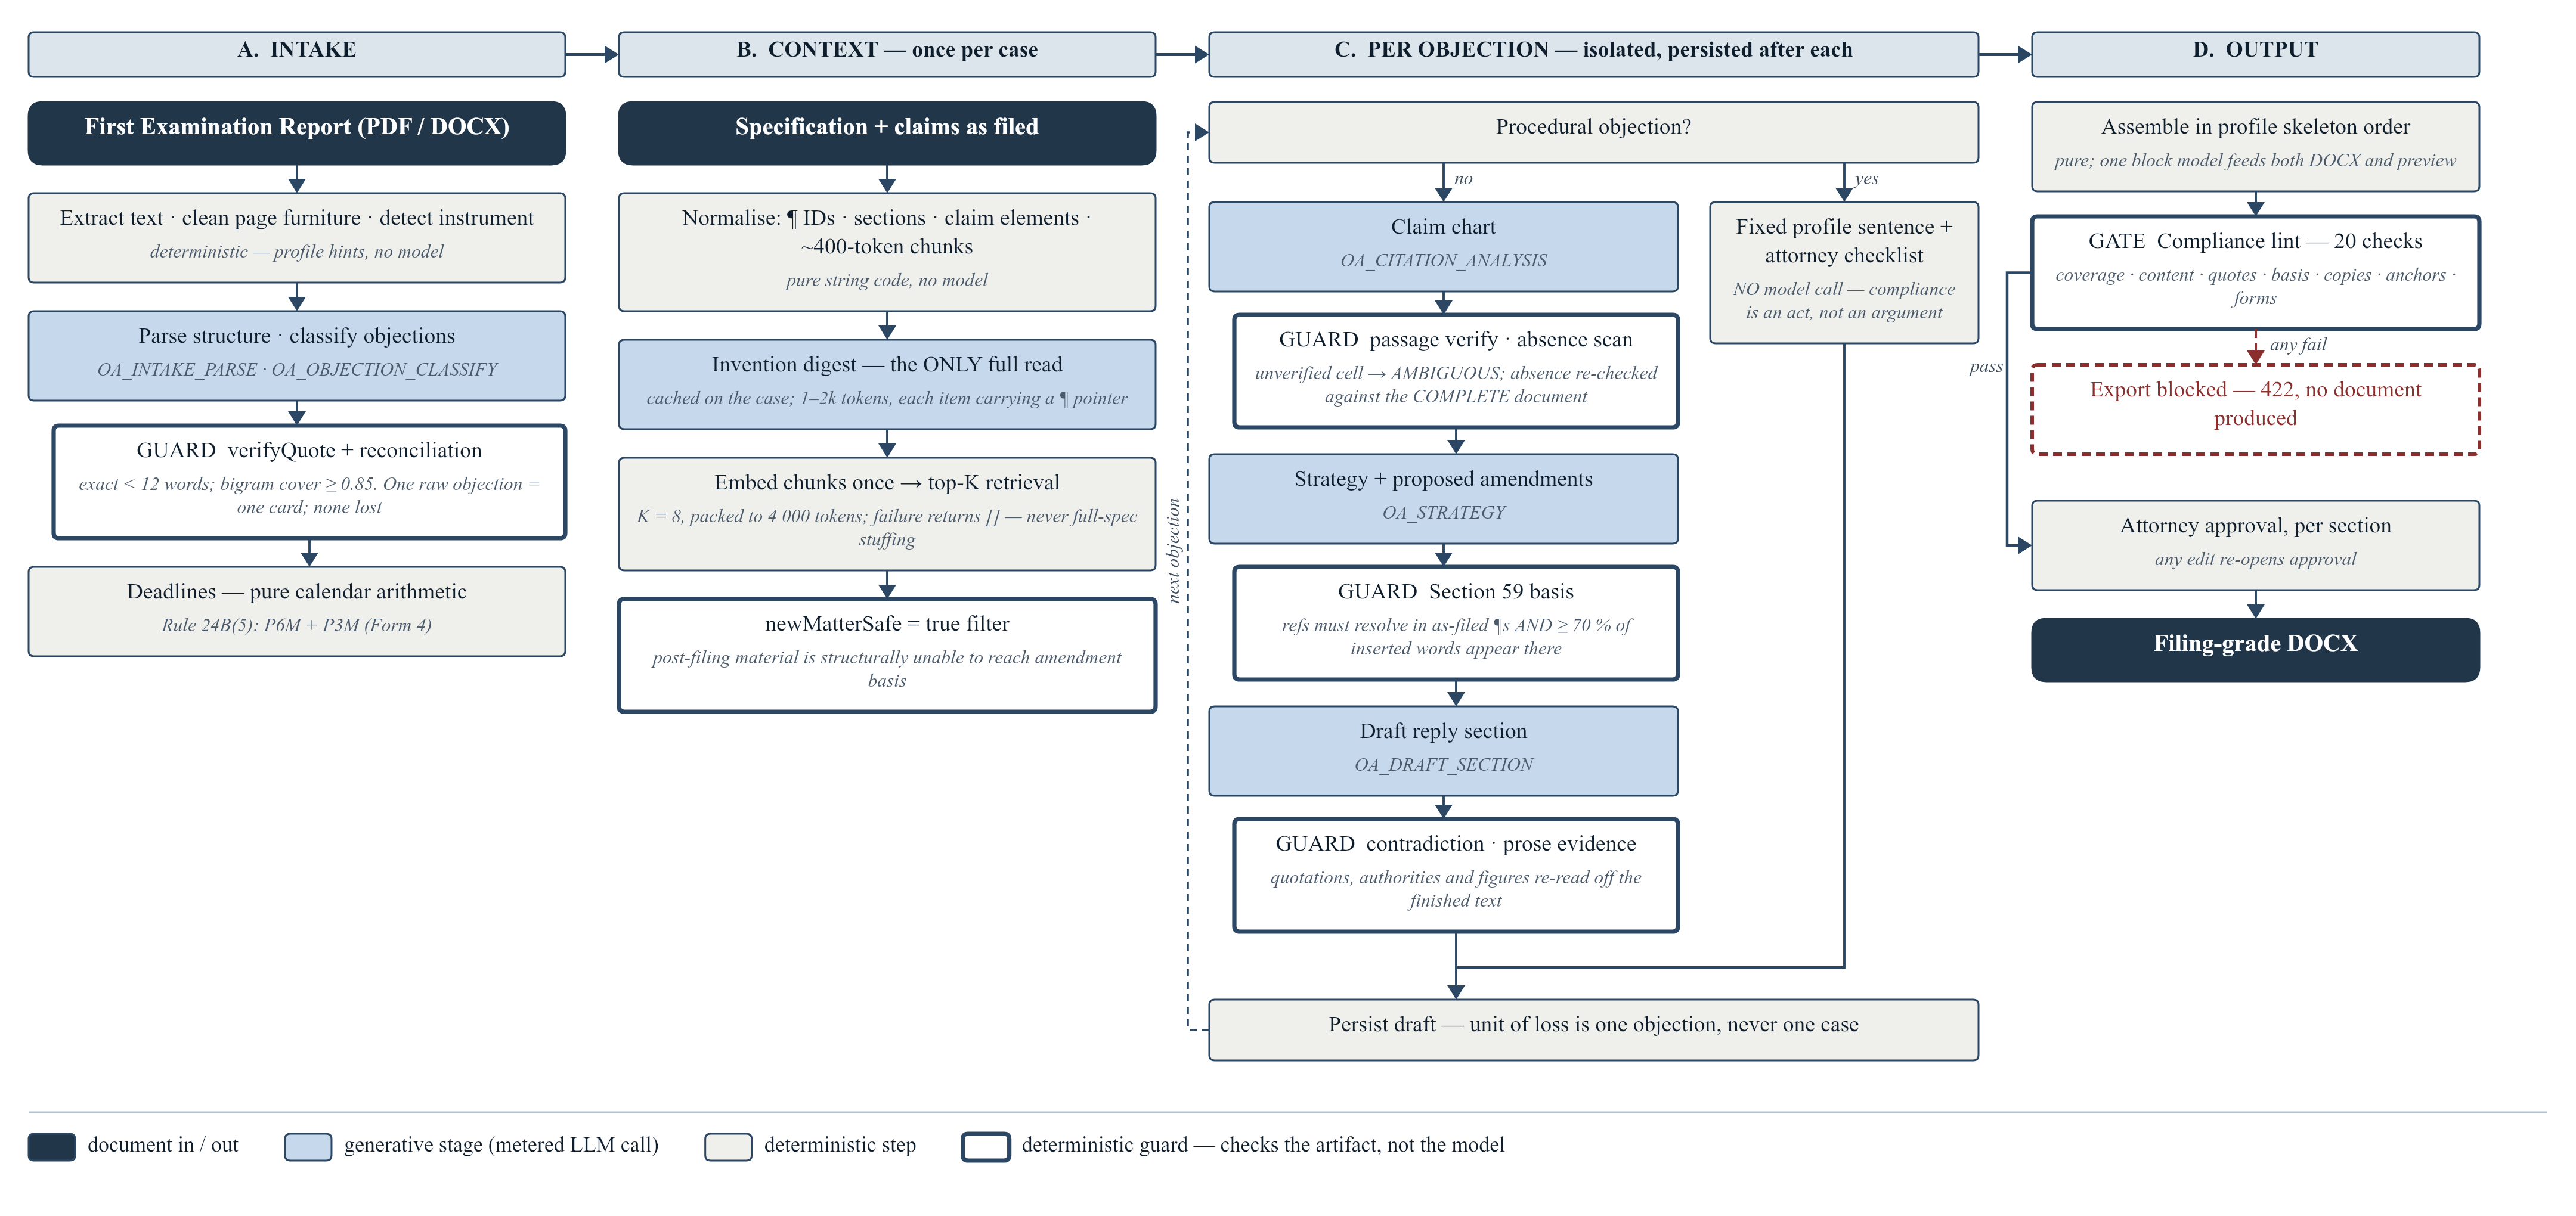
\includegraphics[width=\textwidth]{figures/fig1-pipeline.png}
\caption{The verification-first FER pipeline. Generative stages (mid-tone) are each followed by a deterministic guard (heavy rule) that checks the produced artifact rather than asking the model to attest to it. Procedural objections bypass generation entirely, because compliance is an act rather than an argument. The compliance lint is a blocking gate: on any failure the export returns 422 and no document is produced.}
\label{fig:pipeline}
\end{figure*}

\subsection{Intake}

Ingestion is triggered by a PDF, DOCX or text upload. Raw bytes are format-detected by magic bytes and converted to text; a scanned PDF with no extractable text layer is rejected with a clear error rather than silently producing an empty document.

The extracted text then passes through a \textbf{furniture cleaner}. This step is not cosmetic. PDF-to-text conversion injects repeated running headers, page-number footers, and---at every page break---a duplicate of the final line before the break repeated after it. Those artifacts sever sentences, and a severed sentence defeats exact quote matching downstream. Cleaning reconnects the prose so that the model's verbatim quotes can actually be found in it. The cleaned text is what is stored and what all later verification matches against.

\textbf{Instrument detection is deterministic}: profile detection hints are matched as substrings, the instrument with the most hits wins, and confidence is reported as the hit ratio. No model is involved in deciding what kind of document arrived.

A parsing call then extracts dates, parties, cited documents and objections, copied verbatim. The parsing prompt carries one office-specific negative instruction worth noting: it explicitly forbids inferring objections from the Indian FER's Part~I summary grid, because the polarity of that grid's yes/no answers differs from row to row and is unreliable. Objections must come from the Part~II detailed observations and the Part~III formal requirements. This is knowledge about \emph{reading the document}, not about the law, which is why it lives in the prompt rather than the profile.

Trigger dates pass a strict ISO guard---permissive date parsing accepts ambiguous formats such as \code{10/13/2025} and silently produces the wrong deadline---and deadlines are then computed by a \textbf{pure calendar function} from the profile rules, with month arithmetic clamped to month ends so that a six-month period from 31~August ends on 28 or 29~February rather than overflowing into March.

\subsection{Citation Resolution}

Resolving a cited document to full text is a cost-ordered cascade, run as a background job: the local corpus first (free and instant, accepted only if the record holds both claims and description), then an authoritative open patent-data service for European and international numbers, then a public patent page, and only as a last resort a paid retrieval service. Non-patent literature and citations without a document number short-circuit to a manual-upload state.

One implementation detail is load-bearing. Every database write in this cascade is guarded on the row still being in the pending state. Retrieval takes seconds per document, and within that window the attorney may have uploaded their own copy; an unguarded write would stamp a resolved citation back to ``manual required''.

\subsection{Reply Preparation}

The preparation run is the core of the module. Because a real FER requires roughly three model calls per objection and can take from several minutes to an hour, the endpoint never performs the work inside the request. It enqueues a job, returns immediately, and the client polls for status.

The run has four phases.

\emph{1) Invention context, computed once per case.} The specification is normalised---paragraph identifiers, canonical sections, claim elements and overlapping chunks---entirely in pure string code with no model involvement. A cached digest is reused if present; otherwise one digest pass distils the problem, solution, key features, technical advance, efficacy data and independent-claim elements, each carrying a paragraph pointer so the digest remains citable. Only a genuine digest is ever persisted, because writing an empty fallback would defeat the null check that triggers rebuilding.

\emph{2) Draft row opened before any work begins.} If a previous run died mid-way, its row is resumed rather than superseded. Opening a new version would make it the latest draft the workspace renders, blanking sections the attorney could already see, and would re-purchase every model call behind the objections already drafted. Only sections that actually contain text are carried over, so a retry replaces a failure instead of sitting beside it.

\emph{3) Per-objection loop, each iteration isolated and persisted.} For each objection the run checks whether a pause has been requested, routes procedural objections to a non-generative path, builds a claim chart if the objection cites documents whose full text is available, produces strategy options with an amendment-basis check, drafts the reply section, and persists. Each objection is wrapped in its own error boundary: a stage that throws costs \emph{that objection} its section---recorded explicitly so the attorney can see which one needs writing and so a later run retries only that one---and never the remainder of the run.

\emph{4) Named sections.} Preliminary submissions and the conclusion and prayer are drafted last, and the draft is marked complete.

The shape of this loop exists to protect already-purchased model output. The unit of loss is one objection, never one case.

\subsection{The Model Runner Contract}

Every generative call in the module passes through a single function. There is no second path. Prompt assembly is fixed and three-part: a jurisdiction-agnostic global instruction for the stage, then the profile's jurisdiction overlay for that stage, then the input block, then a demand for a single JSON object. Output parsing is tolerant of code fences and surrounding prose.

Two properties of this contract matter more than the rest. First, every call is metered through a central gateway with a task and stage code, so model selection, quota, plan entitlement and usage recording are uniform, and the gateway is injectable for testing without a database or API keys. Second---and this is the module's single most important resilience property---\textbf{failures are returned as data, not thrown}. Both a gateway exception and a gateway failure response produce a typed failure result, and the caller decides the blast radius. A single throw crossing the per-objection boundary would previously abort an entire run.

%==============================================================================
\section{The Verification Layer}
\label{sec:verification}

This section describes the module's principal contribution: the deterministic checks that stand between generated text and a filed document. Each is a pure function or a query predicate. None calls a model.

\subsection{The Grounding Primitive}

\code{verifyQuote} answers one question: does this quoted span actually appear in that source document? It is used for examiner quotations, for claim-chart passages and, transitively, in the export gate.

Matching operates on a folded form of both strings: Unicode NFKC normalisation to resolve superscripts and ligatures, unification of dash, quotation-mark and non-breaking-space variants, whitespace collapse, and lower-casing. Words are preserved, so folding absorbs extraction noise without weakening the test. Verification then proceeds in the tiers shown in Table~\ref{tab:verify}.

\begin{table}[h]
\caption{Tiers of the grounding primitive}
\label{tab:verify}
\centering
\footnotesize
\renewcommand{\arraystretch}{1.2}
\begin{tabular}{@{}ll@{}}
\toprule
\textbf{Condition} & \textbf{Result} \\
\midrule
Exact folded substring & verified \\
Needle shorter than 12 words & \emph{not} verified \\
Consecutive word-bigram coverage $\geq 0.85$ & verified \\
Otherwise & \emph{not} verified \\
\bottomrule
\end{tabular}
\end{table}

The design of the third tier is the interesting part. A verbatim examiner quotation may run to two thousand characters, and a single stray superscript or OCR glitch inside that span would defeat exact matching. Bigram coverage tolerates such damage. It does not tolerate fabrication, because the consecutive word pairs of an invented sentence are simply absent from the source. Short quotations are held to exact matching precisely because bigram coverage becomes unreliable at small lengths.

\subsection{Objection Reconciliation}

Classification assigns canonical codes, but the code then enforces an invariant the model cannot be trusted to maintain: \textbf{every raw parsed objection produces exactly one card}. An explicit index binds each model output to a raw objection. A repeated index is treated as a duplicate and is not permitted to consume a different raw objection, which would otherwise mark an unrelated objection as answered. Positional fallback applies only when no usable index is supplied. Any raw objection the model dropped is appended as an \code{OTHER} card carrying a ``review and re-categorise'' rationale. An unknown code is coerced to \code{OTHER}. Where the model's copy of the examiner text has drifted but the raw parse verifies, the raw text wins.

Complete classification failure is not fatal. Deterministic fallback cards are built straight from the parse, and the route returns a warning rather than an error. \textbf{No objection is ever lost}, because an unanswered objection in a filed reply is the module's worst possible defect.

\subsection{Claim-Chart Passage Verification}

Every chart cell marked as disclosed must carry a passage that verifies against the cited document's stored text. A cell whose passage does not verify is \textbf{downgraded to ambiguous} and the passage is discarded---the model's conclusion is not accepted merely because it was stated.

A second filter operates before charting begins: only citations whose resolved text actually contains claims or a description are charted at all. Charting a bare title and abstract produces false ``not disclosed'' distinctions, and those distinctions are exactly what the attorney would rely on to argue novelty.

\subsection{Full-Document Absence Verification}

This check addresses a failure that grounding alone cannot reach. To keep prompts affordable, the charting stage sees only the first six thousand characters of each cited document, while a patent specification runs from fifty thousand to two hundred thousand. The model therefore returns ``not disclosed'' for text it was never shown---and that verdict is then filed as a statement of fact to the Controller.

Before any absence verdict is trusted, the \textbf{complete stored document} is scanned for the claim feature. No embeddings, no additional model call; the full text is already on file, and only the prompt was truncated.

Two properties make the check usable in practice. It is \textbf{deliberately asymmetric}: a hit downgrades the verdict to ambiguous and shows the attorney the passage, whereas a miss upgrades nothing. One passage proves disclosure; no passage proves nothing. And it suppresses \textbf{generic field vocabulary}. Without that suppression, a feature such as ``a sensor coupled to a processor configured to output a control signal'' matched almost any electronics citation on a single common word, overturned genuine absence findings, and thereby emptied the chart's distinction list---costing the reply its novelty argument. The suppression list covers both classical patent boilerplate and the everyday vocabulary of software, electronics and biotechnology.

\subsection{Post-Draft Contradiction Lint}

The absence scan prevents the chart from being wrong; the contradiction lint prevents the prose from contradicting a chart that is right. A drafted section can state that a document ``does not disclose the phaseolin promoter'' while the chart for that same document records the feature as disclosed. Nothing upstream catches this: the sentence is fluent, names a real document, and quotes nothing that requires verification.

Because mapping a free-text sentence to a claim limitation is easy in some cases and unreliable in others, the lint reports a confidence tier and only a \textbf{high-confidence} mapping may block a filing. A sentence that carries several limitations, several document labels or unresolved pronouns, or that argues about the examiner rather than about a document, is surfaced to the attorney rather than treated as an error. An absence asserted against a document that is not completely on file blocks regardless of tier, since that finding does not depend on resolving which limitation the sentence meant.

\subsection{Evidence Checks Over the Drafted Prose}

Everything discussed so far verifies \emph{structured} output. The thing actually filed, however, is free prose. Three deterministic checks read the finished text back.

\begin{itemize}
\item \textbf{Quotations.} Any quoted span of meaningful length attributed to a document on file must verify against that document. A fabricated quotation blocks. An unlocatable quotation with no attribution warns rather than blocks, and quoted \emph{claim terms} are correctly excluded from treatment as quotations of a document.
\item \textbf{Authorities.} Case names appearing in the prose are checked against the whitelist for that objection and its doctrine. A United States authority in an Indian reply blocks. Short-form citations of a whitelisted case pass. Where a jurisdiction whitelists no authority for an objection, citing any authority blocks.
\item \textbf{Figures.} Numerical technical effects asserted in the reply must appear in material on the record. Claim numbers and paragraph numbers are explicitly excluded so that ordinary cross-references are not mistaken for experimental data.
\end{itemize}

All three are calibrated for \textbf{precision over recall}, on the stated reasoning that a check which fires on correct replies is switched off within a week and thereafter catches nothing at all. Each also distinguishes ``skipped because nothing is on file'' from ``passed'', so an empty record never reads as a clean result.

\subsection{The Section 59 Guard}

Amendment basis is protected at two levels.

\textbf{Structurally}, the retrieval query that finds candidate basis paragraphs carries the predicate \code{newMatterSafe = true}, and that flag is set only for the as-filed specification and claims. Post-filing evidence---comparative efficacy data, expert declarations, teaching-away references---is therefore \emph{incapable} of reaching the basis finder. It is not discouraged from doing so; it cannot be retrieved. Supplementary material travels on a separate, explicitly labelled channel usable for argument and evidence only.

\textbf{Textually}, each proposed amendment is checked as follows. Cited basis references are resolved against the as-filed paragraphs, tolerating the several formats the drafting stages actually emit---including ranges such as \code{\P0038--\P0041}, which retrieval itself produces as chunk labels and which a naive lookup rejected, causing valid amendments to be silently dropped. Every inserted span is then tokenised, short tokens are discarded, and at least \textbf{70\,\%} of the remaining words must appear in the cited paragraphs. Falling short marks the amendment as failed, and a failed amendment cannot enter the reply.

The guard also encodes a point of law. A \textbf{deletion requires no basis}: Section 59 governs what may be added, so cancelling a claim or striking words introduces no new matter. Reporting such an amendment as ``without basis'' told the attorney that a perfectly valid narrowing amendment was legally defective. Where some references resolve and others do not, the verdict is partial---real textual support, but a combination the attorney must stand behind personally.

\subsection{Case-Law Scoping}

Only the authorities whitelisted for the specific objection, together with its doctrine's leading cases, are supplied to the drafter, and entries tagged to a sub-clause are dropped when the sub-clause is known. When the list is empty, that fact is stated \textbf{explicitly} in the prompt---``cite no case law''---because silence would leave the model free to fall back on half-remembered case names. The list that feeds the prompt is the same list that feeds the post-hoc check, which is itself covered by regression tests.

\subsection{Procedural Bypass}

Formal objections never reach a model at all. A Form~3 statement under Section 8, an annexure, a declaration of biological source \cite{bda2002}, an NBA approval---these are \textbf{not argued; they are done}. A model can only \emph{assert} that the act took place, and an asserted compliance that did not occur is a misrepresentation to the Controller over the attorney's signature.

Objections marked procedural in the profile therefore route to a deterministic builder that emits a fixed reply sentence drawn from the profile, plus an action checklist rendered for the attorney and \textbf{never filed as prose}---the profile's action entries are full of conditionals and practice notes, and a reply reciting one would be a leaked worksheet rather than a submission. The paragraph is flagged, and the DOCX renderer honours the flag by highlighting it and appending an explicit ``remove before filing'' marker. As a secondary benefit, this saves two paid calls per formal objection.

\subsection{The Blocking Compliance Gate}

Export is gated. The lint runs twenty distinct checks, of which the following block the export outright: every non-dismissed objection has an approved reply; no approved section is empty; every approved reply rests on a verified examiner quotation; every amended claim cites specification basis; that basis resolves in the as-filed text; the specification designated as-filed actually exists on the case; marked and clean claim copies carry identical claim-number sets; every paragraph reference in the filed text resolves; no internal anchor residue survives into the document; prior-art statements do not contradict the chart at high confidence; quotations, authorities and asserted figures pass the prose checks; and, where the report raises a Section 8 objection, the attorney has \emph{positively confirmed} the Form~3 position---because on a procedural objection, \textbf{silence is not compliance}. Warning-level checks cover FER ordering, power of attorney, Form~4, applicant name and stated-versus-computed deadline agreement.

A failing lint returns an error status and no document is produced. The lint result is persisted either way, so the record shows what was checked and when.

%==============================================================================
\section{Context and Cost Architecture}
\label{sec:cost}

\subsection{The Naive Baseline}

A specification runs from twenty thousand to eighty thousand tokens. Sending it to every stage of every objection---six objections across three generative stages at a fifty-thousand-token specification---costs roughly \textbf{900\,000 input tokens per case} before citations or revisions are considered. At reasoning-model rates, that is a material sum spent repeatedly re-reading one document, multiplied by every run and every revision.

\subsection{Three Levers}

\emph{Lever 1---the digest.} One pass over the paragraph-numbered specification produces a compact structured summary of one to two thousand tokens, each element carrying a paragraph pointer so it remains citable. It is cached on the case. Where the case is linked to an existing drafting project inside the platform, the same structure is assembled from already-normalised data for \textbf{zero model tokens}.

\emph{Lever 2---retrieval instead of stuffing.} All structural work---paragraph identifiers, canonical sections, claim elements, and roughly four-hundred-token chunks with one-paragraph overlap, each labelled with its paragraph range---is done in pure string code. Each chunk is embedded once at intake. Every subsequent stage that needs specification detail issues a top-$K$ approximate nearest-neighbour retrieval \cite{malkov2020} with $K=8$ packed to a four-thousand-token ceiling, filtered by document kind and by the new-matter flag.

Two details in this path repay attention. The query is embedded with a \emph{query-side} embedding request: the embedding model in use is asymmetric, and embedding a query as though it were a document silently degrades retrieval without producing any error. And \textbf{any retrieval failure returns an empty result}, so callers degrade to digest-only context---never to full-specification stuffing, which would convert a retrieval outage into a cost incident.

\emph{Lever 3---skip work that is not needed.} No chart is built when an objection cites nothing, or cites nothing whose full text is available. Procedural objections skip both charting and strategy. Claims and drawings documents are marked as not requiring indexing, because nothing retrieves them; claims reach the charts whole from a dedicated field.

\subsection{Estimated Effect}

Table~\ref{tab:cost} sets the two designs side by side. These figures are \textbf{analytical estimates derived from the token model}, not measurements from production traffic; the module also exposes a deliberately conservative pre-flight estimator so an attorney sees a bound before authorising a run. Because the digest and jurisdiction guidance form a stable prompt prefix across a case's objections, provider-side prompt caching discounts the shared portion on every objection after the first.

\begin{table}[h]
\caption{Estimated per-case input budget (six objections, 50k-token specification)}
\label{tab:cost}
\centering
\footnotesize
\renewcommand{\arraystretch}{1.25}
\begin{tabular}{@{}>{\raggedright\arraybackslash}p{0.24\columnwidth}>{\raggedright\arraybackslash}p{0.30\columnwidth}>{\raggedright\arraybackslash}p{0.34\columnwidth}@{}}
\toprule
\textbf{Item} & \textbf{Naive} & \textbf{This architecture} \\
\midrule
Understanding the invention & $50\mathrm{k}\times6\times3 \approx 900\mathrm{k}$ & one digest pass $\approx55\mathrm{k}$ in, $2\mathrm{k}$ out \\
Per-objection generation & \emph{(included above)} & $6\times(2\mathrm{k}+3\mathrm{k}+1\mathrm{k})\approx36\mathrm{k}$ in \\
Citations & full text, every reference & examiner pinpoints; fetch on demand \\
Embedding & --- & whole specification once \\
\midrule
\textbf{Input tokens} & \textbf{$\approx900\mathrm{k}$} & \textbf{$\approx90$--$100\mathrm{k}$}, mostly cacheable \\
\bottomrule
\end{tabular}
\end{table}

%==============================================================================
\section{Human Oversight and Reliability}

\subsection{Attorney-in-the-Loop Surfaces}

The system files nothing. Every generated section is a draft behind an approval gate, and approval is per section. Four controls define the workflow.

\begin{itemize}
\item \textbf{Objection triage.} An objection card may be confirmed or dismissed. Dismissed objections are excluded from the run and from lint coverage, which is how an attorney disposes of an objection they judge inapplicable without leaving a coverage failure.
\item \textbf{Editing re-opens approval.} Any text edit sets the section back to unapproved. An edited section must be read again before it can be exported.
\item \textbf{Directed redrafting.} A single section can be redrafted with the attorney's own instruction. The current section text and the remark are supplied together, with the remark positioned last---closest to the task---and framed as binding: follow it exactly, keep what works, stay within the supplied evidence and authorities, and if it cannot be done on this record, say so plainly rather than inventing support. The remark is stored on the section as the record of why the wording changed, and the result always returns unapproved, because it has not been read yet.
\item \textbf{Pause and resume.} A stop request is honoured \emph{between} objections, never mid-stage, so a pause never lands inside a paid call or leaves a half-written section. This is the mechanism that lets an attorney interrupt a run, upload a cited prior-art document they hold, and continue with that document in play for the objections not yet drafted.
\end{itemize}

Progress narration is treated as a product surface rather than as logging. Messages describe real work---``Objection 3 of 7 $\cdot$ Inventive step---charting the claims against D1, D2''---and every number in them is read off the case rather than estimated.

\subsection{Reliability Engineering}

The job worker uses a database-lease pattern: candidates are selected and then claimed by a guarded conditional update, so exactly one worker wins under concurrency. A heartbeat renews the lease every sixty seconds, and a worker that loses its lease abandons the job rather than competing with its new owner. Two runtimes share one queue---a standalone worker and an in-process drain---which the lease makes safe. Retries follow a one-minute, five-minute, fifteen-minute backoff to a default of three attempts.

One defect fixed here is worth recording because it is characteristic of long-running LLM pipelines. A preparation run spans minutes to an hour of gateway calls, while the default session credential expired after fifteen minutes, causing every stage after that point to fail with an unrelated-looking tenant-resolution error. The run now mints a ninety-minute internal credential and re-mints it every ten minutes, mutating the shared header object in place so that the refresh reaches calls already in flight further down the pipeline.

Completion notification is sent only by the worker that actually recorded the outcome, so a lease handover cannot produce a duplicate, and only on genuine completion or final failure---never on a retry and never on a deliberate pause. The notification carries the soonest live deadline, because the statutory clock runs whether or not the run succeeded.

%==============================================================================
\section{Implementation Status and Validation}

\subsection{Status}

The module comprises roughly 8\,300 lines of TypeScript across thirty-one stage and infrastructure files, plus the workspace interface and nine HTTP endpoints. It is deployed within a commercial patent-workflow platform. The \textbf{Indian profile is the implemented jurisdiction}, covering the Section 59 basis guard, Rule 24B deadlines, the Section 3(d) and 3(k) sub-clauses, and the Form~3 / Section 8 procedural track. The profile schema already models the deadline shapes required for the United States, European, Australian, New Zealand and United Kingdom offices under three prosecution models---per-report, acceptance-clock, and hybrid---so those jurisdictions are authoring work rather than engineering work.

\subsection{Regression Suite}

The verification layer is protected by \textbf{48 regression tests across two suites, all passing} at the time of writing. Their organisation is itself informative, because each test encodes a defect that reached a draft:

\begin{itemize}
\item paragraph anchors never reach a filing unvetted, and the preview shows the same verdict as the filing;
\item the filed document contains only what the attorney approved, and a failed section never produces a heading with no body;
\item a font name drawn from a jurisdiction profile cannot close the stylesheet and inject script into the preview;
\item claim parsing survives spaced claim markers, numberless back-references and dependencies declared late in a claim;
\item chunking is bounded even for text containing no sentence punctuation;
\item common engineering vocabulary does not overturn a genuine absence finding, while a genuinely distinctive term does;
\item a deletion-only amendment requires no basis, an unsupported insertion is still rejected, and a range basis reference is cited in full rather than truncated to its first number;
\item deadlines are computed relative to today rather than to the ingest date, however they were stored;
\item malformed model output cannot fail an entire ingest;
\item a fabricated quotation blocks while a genuine one passes; a foreign authority blocks while a whitelisted one passes in both full and short form; an invented technical effect blocks while a figure present in the specification passes;
\item and each prose check is \emph{skipped} rather than \emph{passed} when nothing is on file.
\end{itemize}

\subsection{What We Do Not Claim}

We report no accuracy, acceptance-rate or attorney-time figures. Establishing them properly requires a controlled study over a corpus of real FERs with blinded expert assessment of the resulting replies, together with grant-outcome tracking over the prosecution cycle, and that study has not yet been conducted. We think it important to say so plainly: the contribution offered here is an architecture and a verification methodology, evidenced by the implemented guards and the regression suite that protects them, and not an empirical claim about output quality.

%==============================================================================
\section{Discussion and Limitations}

\subsection{What the Architecture Buys}

The design converts a class of unbounded risks into bounded ones. A model that fabricates an examiner quotation produces a card flagged as unverified, which blocks export. A model that invents disclosure in a cited document produces a chart cell downgraded to ambiguous. A model that proposes an amendment without support produces a failed verdict, and the amendment never enters the reply. A model that reaches for a familiar foreign authority produces prose that the whitelist check rejects. In each case the failure surfaces as a visible, named, blocking condition rather than as a confident sentence in a filed document.

Equally important, the design bounds \emph{economic} loss. Work is persisted after every objection; a crash costs one objection, not one case. A dead run resumes rather than reopening, so previously purchased output is not re-purchased. Stage failures are data rather than exceptions, so one bad objection does not abort six good ones.

\subsection{Limitations}

\textbf{Precision--recall calibration.} The prose checks are explicitly tuned for precision. This is the right trade-off for a gate that attorneys must be willing to keep switched on, but it means some fabrications will pass. The checks reduce the rate; they do not reduce it to zero.

\textbf{Truncated charting evidence.} Charting still sees only the first six thousand characters of a cited document. The absence scan corrects false absences afterwards, but a disclosure buried deep in a long specification may simply never be found in the first place, and no downstream check can create evidence that was not sought.

\textbf{Single jurisdiction in production.} The claim that the engine is jurisdiction-agnostic is supported by the absence of country-code branching and by a schema that models several prosecution structures, but it has been demonstrated end to end only for India. A second profile would test the abstraction properly.

\textbf{No outcome evidence.} As stated above, we have no data linking generated replies to prosecution outcomes.

\textbf{Dependence on text extraction.} A scanned FER with no text layer is rejected rather than processed. Optical character recognition would extend coverage, but it would also introduce noise into precisely the text that all verification matches against, and the interaction between OCR error rates and the bigram threshold would need to be characterised before that is safe.

\subsection{Ethical and Professional Considerations}

The system is designed on the assumption that a qualified patent agent or attorney is the author of the filed document and remains professionally responsible for it \cite{mppp}. Three design choices follow directly. Approval is per section and is revoked by any edit. Procedural compliance is never asserted by a model. And the interface deliberately shows an attorney a patent document rather than the retrieval route that produced it, so that internal machinery does not acquire an unearned appearance of authority. We consider the ``assert compliance'' failure mode the most serious risk in this application domain, which is why it is addressed structurally---by removing the model from that path entirely---rather than by instruction.

%==============================================================================
\section{Conclusion}

Generating a First Examination Report reply is a task where large language models offer real leverage and where their characteristic failure mode is professionally unacceptable. We have described a deployed system that resolves that tension by refusing to trust generated assertions on their own terms. Every stage that generates is followed by code that checks: examiner quotations against the cleaned report, chart passages against the cited document, absence findings against the complete text rather than the truncated prompt, drafted prose against its own chart, amendments against the specification as filed, authorities against a jurisdiction whitelist, and the entire draft against a blocking compliance gate. Formal objections bypass generation altogether, because compliance is an act and not an argument. All local law lives in a validated profile, so the engine holds no jurisdiction-specific logic, and a retrieve-per-need context strategy keeps the cost of that rigour proportionate.

The general lesson we draw is narrow but, we think, transferable to other regulated drafting domains: \textbf{grounding reduces the probability that a model fabricates, but only verification reduces the probability that a fabrication survives.} In a setting where the output is signed and filed with a public authority, it is the second probability that matters.

%==============================================================================
\section*{Acknowledgment}

[To be completed by the authors.]

%==============================================================================
\begin{thebibliography}{00}

\bibitem{act1970} \emph{The Patents Act, 1970} (No.~39 of 1970), Government of India, as amended.

\bibitem{rules2003} \emph{The Patents Rules, 2003}, as amended by the Patents (Amendment) Rules, 2024, Government of India.

\bibitem{dahl2024} M. Dahl, V. Magesh, M. Suzgun, and D. E. Ho, ``Large legal fictions: Profiling legal hallucinations in large language models,'' \emph{Journal of Legal Analysis}, vol.~16, no.~1, pp.~64--93, 2024.

\bibitem{magesh2025} V. Magesh, F. Surani, M. Dahl, M. Suzgun, C. D. Manning, and D. E. Ho, ``Hallucination-free? Assessing the reliability of leading AI legal research tools,'' \emph{Journal of Empirical Legal Studies}, 2025.

\bibitem{krestel2021} R. Krestel, R. Chikkamath, C. Hewel, and J. Risch, ``A survey on deep learning for patent analysis,'' \emph{World Patent Information}, vol.~65, art.~102035, 2021.

\bibitem{lee2020} J.-S. Lee and J. Hsiang, ``Patent claim generation by fine-tuning OpenAI GPT-2,'' \emph{World Patent Information}, vol.~62, art.~101983, 2020.

\bibitem{casola2022} S. Casola and A. Lavelli, ``Summarization, simplification, and generation: The case of patents,'' \emph{Expert Systems with Applications}, vol.~205, art.~117627, 2022.

\bibitem{lewis2020} P. Lewis \emph{et al.}, ``Retrieval-augmented generation for knowledge-intensive NLP tasks,'' in \emph{Proc. Advances in Neural Information Processing Systems (NeurIPS)}, 2020, pp.~9459--9474.

\bibitem{shuster2021} K. Shuster, S. Poff, M. Chen, D. Kiela, and J. Weston, ``Retrieval augmentation reduces hallucination in conversation,'' in \emph{Findings of EMNLP}, 2021, pp.~3784--3803.

\bibitem{ji2023} Z. Ji \emph{et al.}, ``Survey of hallucination in natural language generation,'' \emph{ACM Computing Surveys}, vol.~55, no.~12, pp.~1--38, 2023.

\bibitem{mppp} Office of the Controller General of Patents, Designs and Trade Marks, \emph{Manual of Patent Office Practice and Procedure}, Government of India.

\bibitem{cri2017} Office of the Controller General of Patents, Designs and Trade Marks, \emph{Guidelines for Examination of Computer Related Inventions (CRI)}, Government of India, 2017.

\bibitem{novartis} \emph{Novartis AG v. Union of India}, (2013) 6 SCC 1 (Supreme Court of India).

\bibitem{ferid} \emph{Ferid Allani v. Union of India}, W.P.(C) 7 of 2014, Delhi High Court, 2019.

\bibitem{epc} \emph{Convention on the Grant of European Patents (European Patent Convention)}, Art.~123(2), 16th ed., European Patent Office.

\bibitem{malkov2020} Y. Malkov and D. Yashunin, ``Efficient and robust approximate nearest neighbor search using hierarchical navigable small world graphs,'' \emph{IEEE Trans. Pattern Analysis and Machine Intelligence}, vol.~42, no.~4, pp.~824--836, 2020.

\bibitem{bda2002} \emph{The Biological Diversity Act, 2002} (No.~18 of 2003), Government of India.

\bibitem{usc132} 35 U.S.C. \S132(a), \emph{United States Code}---Notice of rejection; reexamination.

\end{thebibliography}

\end{document}
